\subsubsection*{الف}
توابع first و follow را برای هر یک از غیرپایانه‌ها بدست می‌آوریم:

\setLTR
$
\begin{cases}
	first(S)=first(L)=\{ \ ( \ \}+first(E) = \{ \ , \ ( \ \} \\
	first(L)= \{ \ ( \ , \ \} \\
	first(B)= \{ \ ; \ = \ \} \\
	first(E)= \{ \ a \ ( \ , \ \} \\
	first(J)= \{ \ ) \ \}
\end{cases}
	$

	$
\begin{cases}
	follow(S)=\{ \ ; \ \$ \ \} \\
	follow(L)=first(B)+follow(E)+first(J)= \{ \ ; \ = \ ) \ \} \\
	follow(B)=follow(S)=\{ \ ; \ \$ \ \} \\
	follow(E)=first(J)=\{ \ ) \ \} \\
	follow(J)=first(B)+follow(E)+first(J)= \{ \ ; \ = \ ) \ \}
\end{cases}
$
\setRTL

\subsubsection*{ب}
در این بخش جدول پارس $LL(1)$ مربوط به گرامر فوق را رسم کرده‌ایم:

\qquad\qquad\qquad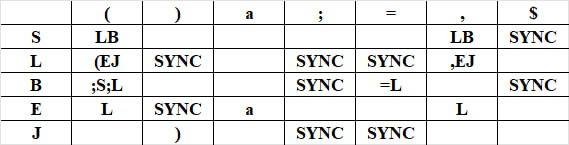
\includegraphics[width=0.7\linewidth]{figs/1.png}

\pagebreak
\subsubsection*{ج}

رشته ورودی ما 
$(a)=(a,(=a))$
است، حال آن را پارس می‌کنیم:


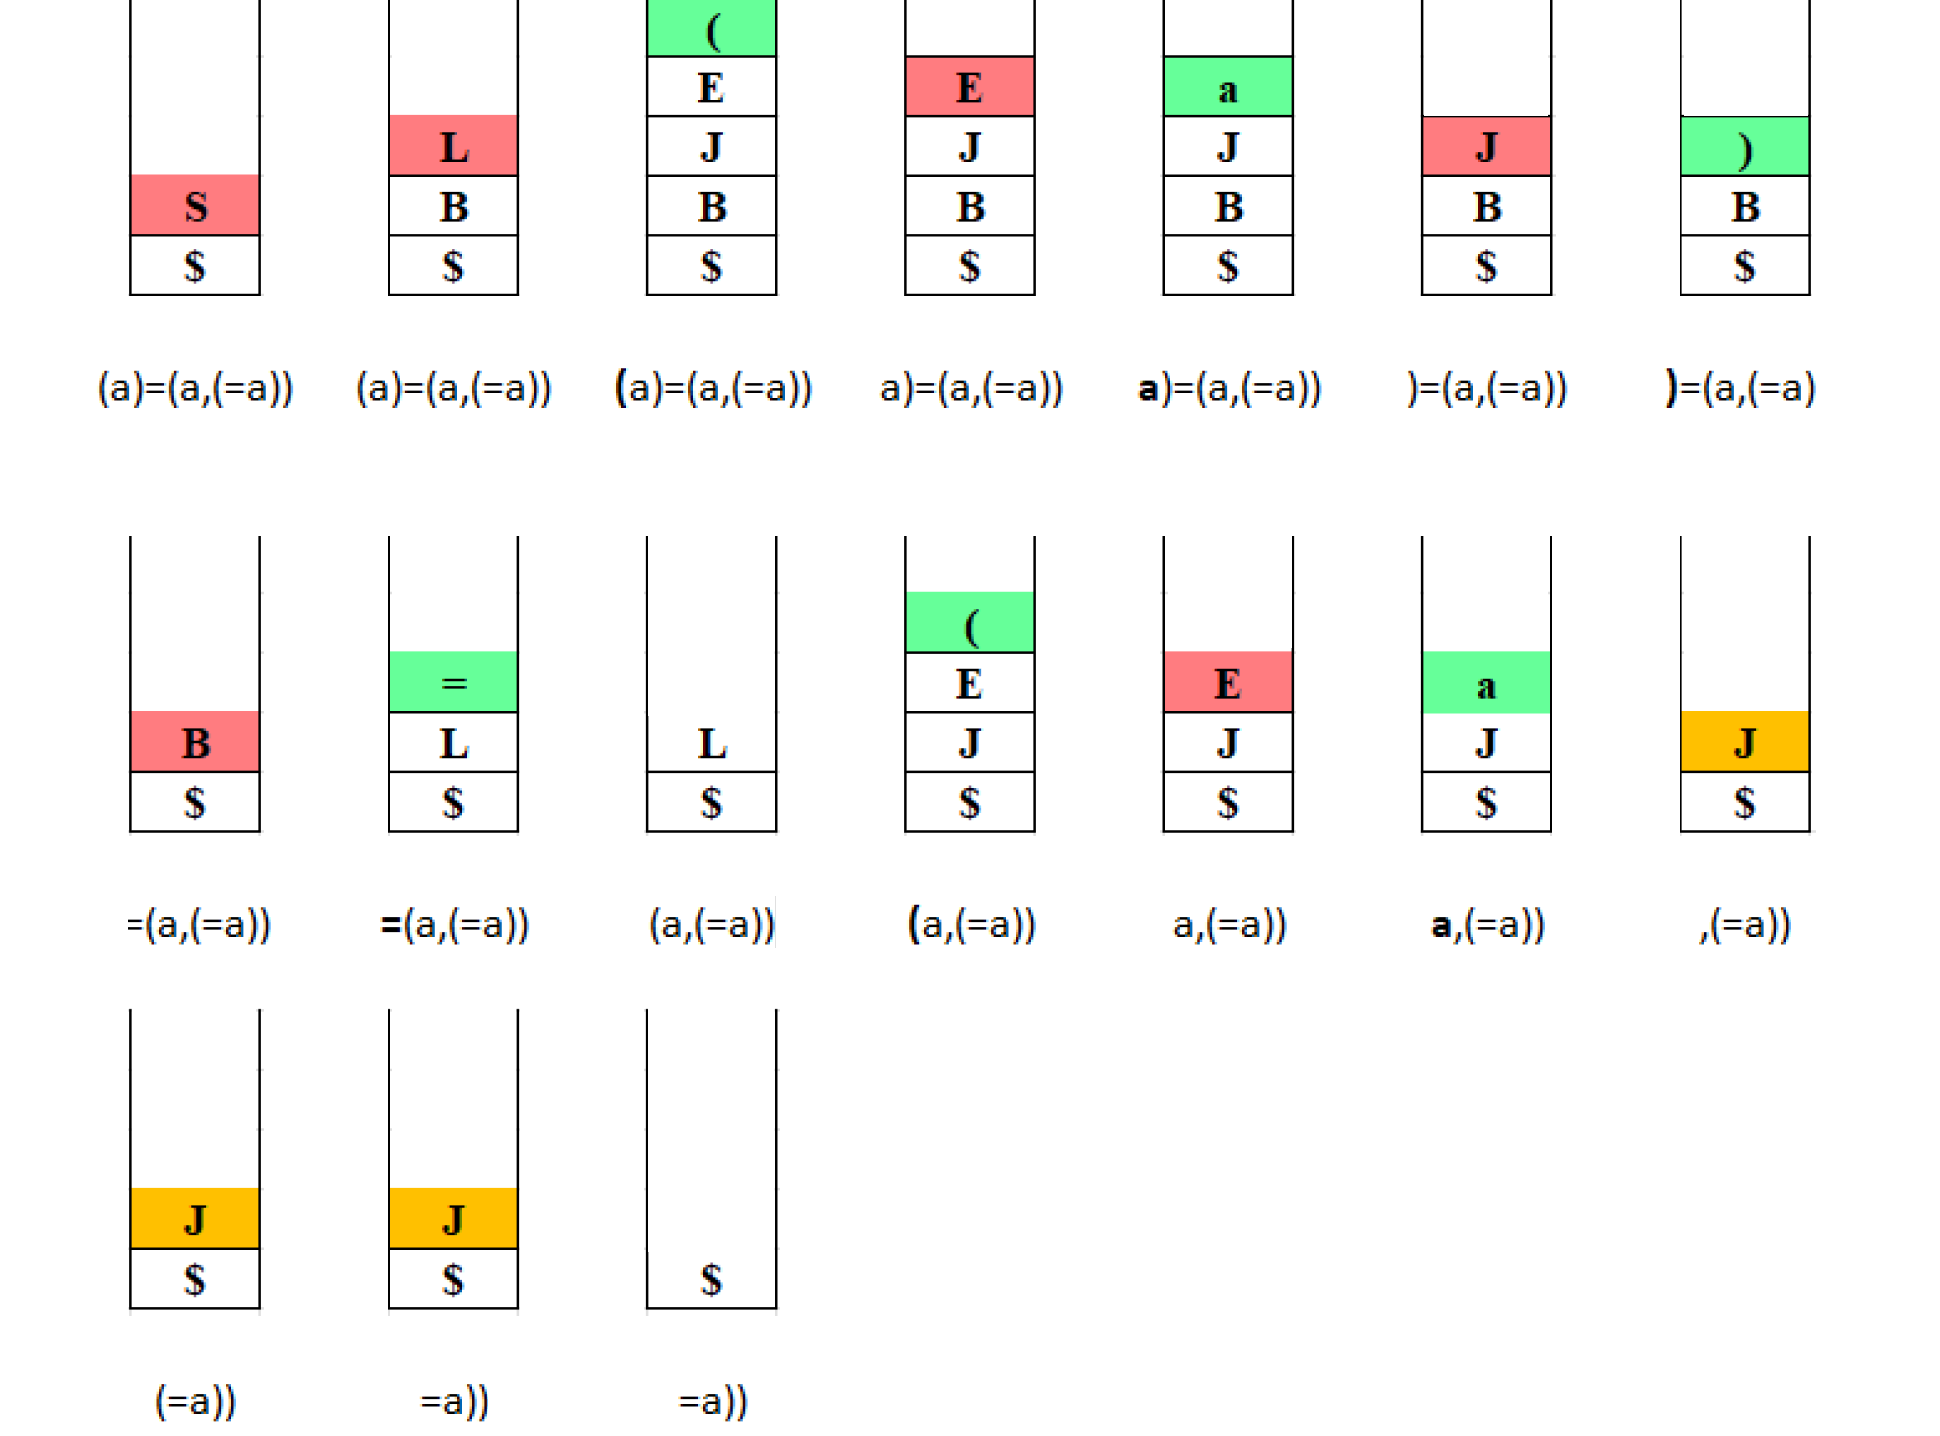
\includegraphics[width=1\linewidth]{figs/2.png}

رشته Match شده‌ی ما
$(a)=(a$
است.

حال مطابق Mode Panic باید رشته باقی‌مانده را دوباره پارس کنیم، اما چون ترمینال‌های موجود در رشته‌ی باقی‌مانده در جدول به S تعلق ندارند، پس ورودی Accept نمی‌شود.









